\documentclass[demo]{report}

\usepackage{blindtext}
\usepackage{geometry}
\usepackage{float}
\usepackage{babel}
\usepackage[most]{tcolorbox}
\usepackage{tikz}
\usepackage{varwidth}
\usepackage{capt-of}
\usepackage[export]{adjustbox}

\tcbset{enhanced,colback=cyan!5!white,colframe=cyan!75!black,fonttitle=\bfseries}

\begin{document}

\begin{tcolorbox}[drop shadow, title=Esempio: misura della carica elettrica,sidebyside,sidebyside align=top,lower separated=false]
    \blindtext
    \tcblower
        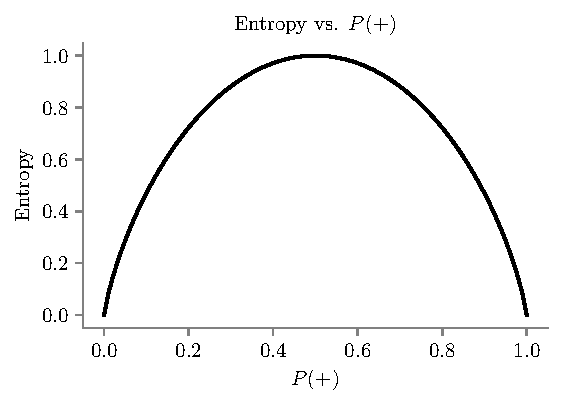
\includegraphics[height=0.6\textheight,width=\linewidth,valign=t]{../figures/decision-trees/entropy.pdf}
        \captionof{figure}{Misura della carica elettrica}\label{fig:fig1}
\end{tcolorbox}

\end{document}